\chapter{Wzmacniacz operacyjny}


\section{Wstępne pomiary}
\begin{itemize}
    \item Na początku należało zapoznać się ze schematem ideowym układu wzmacniacza operacyjnego (\ref{fig:schemat_wzmacniacz_odwracający})
    \item Płytka ze wzmacniaczem:
        \begin{figure}[H]
            \centering
            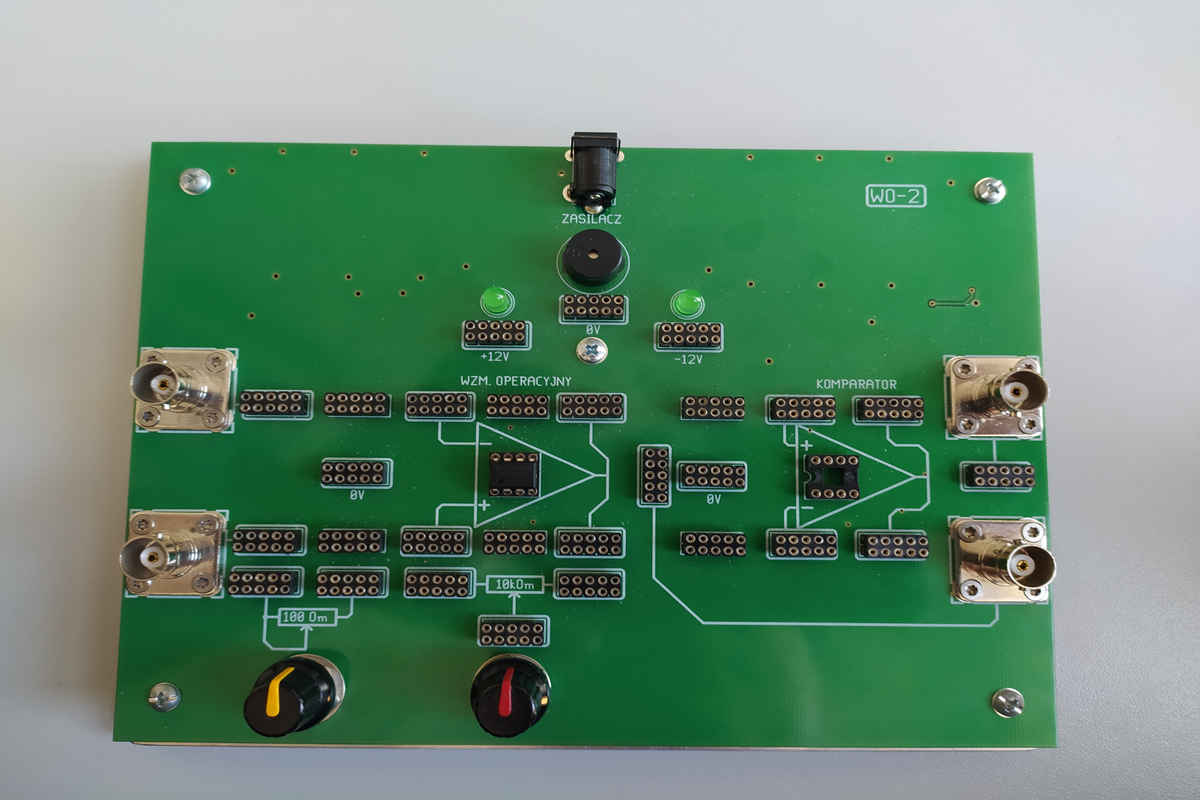
\includegraphics[scale=0.25]{img/phone/1651502036878_scaled.png}
            \caption{}
            \label{fig:my_label}
        \end{figure}
    \item Wartości napięć na pinach +/-:
        \begin{gather}
            \label{pomiar:U+} U_+ = \textbf{11.96V} \\
            \label{pomiar:U-} U_- = \textbf{-12.02V}
        \end{gather}
    \end{itemize}

\section{Budowa układu}
\begin{itemize}
    \item Należało złożyć wzmacniacz o wzmocnieniu \textbf{K = 10}. Zgodnie ze wzorem \ref{wzor:napiecie_wyjsciowe_odwracajacy} należało dobrać odpowiednie oporniki, tak aby ich iloraz $\dfrac{R_2}{R_1}$ = 10.
    \item Dobrano dwa dodatkowe rezystory:
        \begin{gather}
            \label{wzmacniacz:R1} R_1 = \textbf{2.96k}\boldsymbol{\Omega} \\
            \label{wzmacniacz:R2} R_2 = \textbf{32.2k}\boldsymbol{\Omega}
        \end{gather}
        
    \pagebreak
        
    \item Układ złożono korzystając ze schematu (\ref{fig:schemat_wzmacniacz_odwracający}) oraz w/w oporników (\ref{wzmacniacz:R1}, \ref{wzmacniacz:R2}):
        \begin{figure}[H]
            \centering
            \begin{subfigure}[h]{0.4\textwidth}
                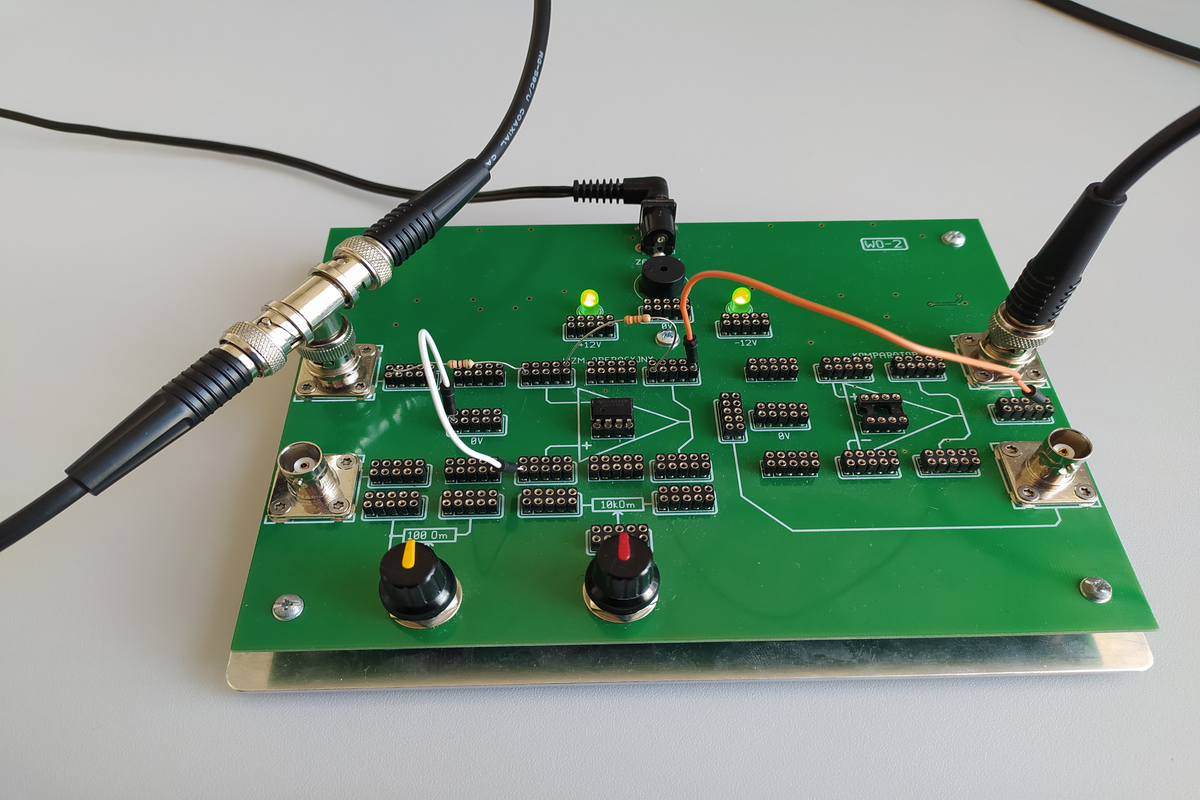
\includegraphics[width=\textwidth]{img/phone/1651502036867_scaled.png}
            \end{subfigure}
            \begin{subfigure}[h]{0.4\textwidth}
                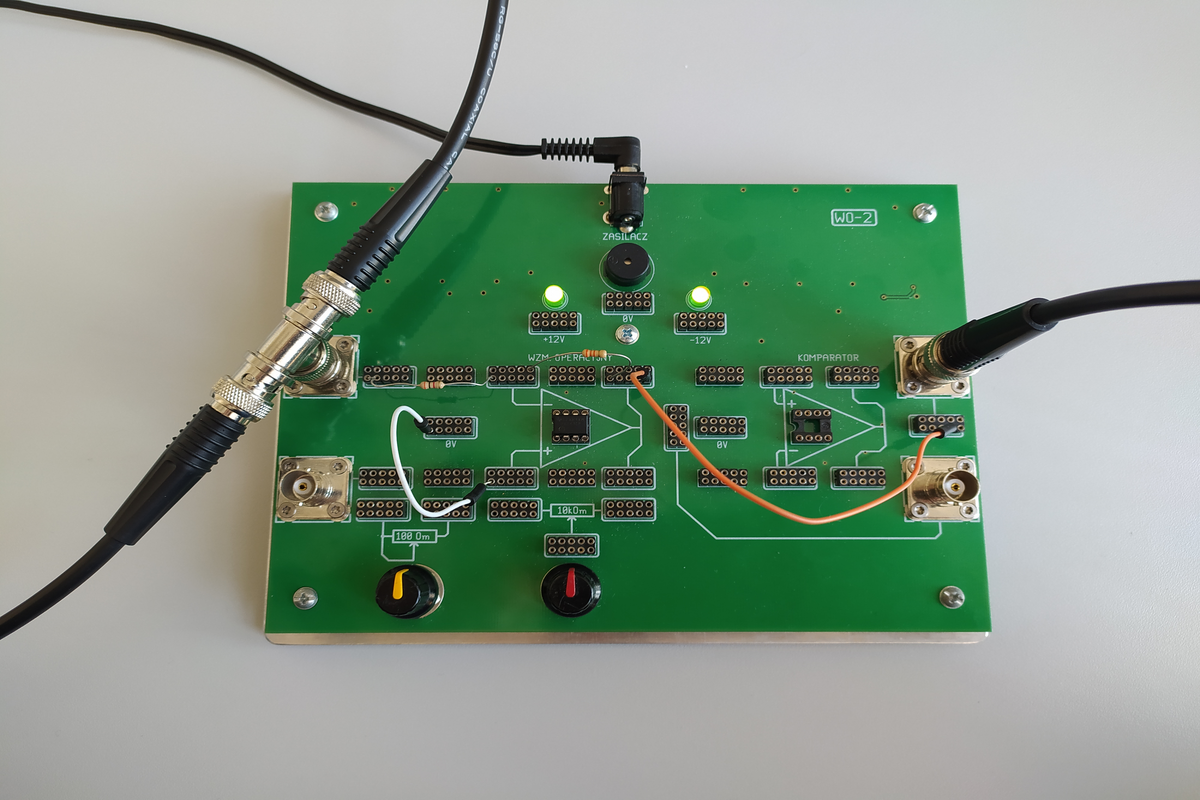
\includegraphics[width=\textwidth]{img/phone/1651502036857_scaled.png}
            \end{subfigure}
            \caption{Zmontowany układ}
            \label{wzmacniacz:zmontowany_uklad}
        \end{figure}
\end{itemize}

\section{Testowanie poprawności układu oraz wartości wzmocnienia}
\begin{itemize}
    \item Za pomocą generatora funkcyjnego przesłano na płytkę falę sinusoidalną o parametrach: \textbf{1kHz} oraz \textbf{1V}. Ten sam sygnał za pomocą trójnika wyprowadzono do \textbf{kanału 1}, wyjściowy sygnał poprowadzono do \textbf{kanału 2}
    \item Odczytane za pomocą funkcji wbudowanych parametry sygnałów na oscyloskopie wyniosły:
        \begin{gather}
            \label{wzmacniacz_parametry:czestotliwosc}f_{we} = 1.003kHz = \textbf{1003Hz} \\
            \label{wzmacniacz_parametry:u_we} U_{we} = 952mV = \textbf{0.952V} \\
            \label{wzmacniacz_parametry:u_wy} U_{wy} = \textbf{10.6V} \\
            \label{wzmacniacz_parametry:przesuniecie}\phi_{12} = \textbf{-162.4}\boldsymbol{\degree}
        \end{gather}
        \begin{figure}[H]
            \centering
            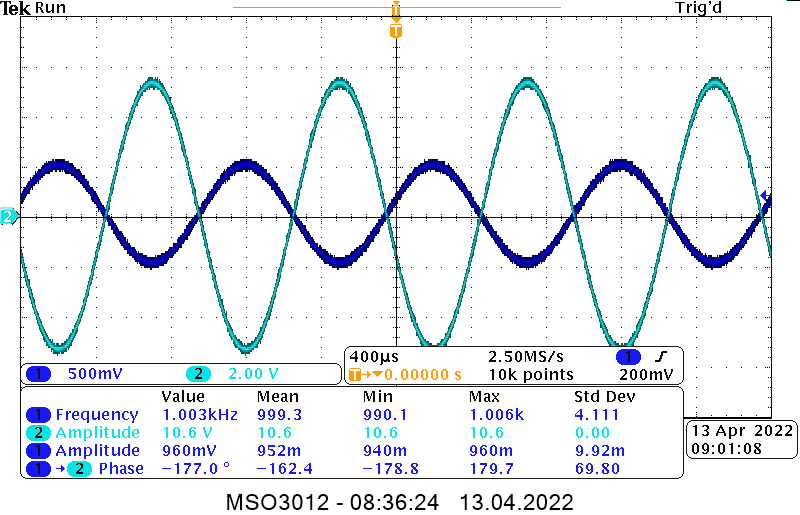
\includegraphics[scale=0.4]{img/osciloscope/dzialajacy_wzmacniacz_cropped.png}
            \caption{}
            \label{fig:dzialajacy_wzmacniacz}
        \end{figure}
    \item Korzystając ze wzoru na teoretyczne napięcie wyjściowe (\ref{wzor:napiecie_wyjsciowe_odwracajacy}) oraz dobranych rezystorów (\ref{wzmacniacz:R1}, \ref{wzmacniacz:R2}):
        \begin{equation}
            K_{teor} = \dfrac{32.2k\Omega}{2.96k\Omega} = \textbf{10.87} 
        \end{equation}
    \item Korzystając z przeprowadzonych pomiarów (\ref{wzmacniacz_parametry:u_we}, \ref{wzmacniacz_parametry:u_wy}):
        \begin{equation}
            K_{eksp} = \dfrac{U_{wy}}{U_{we}} = \dfrac{10.6V}{0.952V} = \textbf{11.04}
        \end{equation}
    \item Sygnał po przejściu przez zbudowany układ (\ref{wzmacniacz:zmontowany_uklad}) zostaje poprawnie wzmocniony (\ref{fig:dzialajacy_wzmacniacz}).
    \item Zgodnie z założeniem sygnał wyjściowy jest przesunięty w fazie względem pierwszego o \textbf{162.4}$\boldsymbol{\degree}$
\end{itemize}

\section{Charakterystyka częstotliwościowa}

\begin{itemize}
    \item Eksperymentalnie wyznaczono wartość częstotliwości $\mathbf{f_g}$ dla której sygnał wyjściowy jest dużo \textbf{niższy} od wejściowego i wyniósł:
        \begin{center}
            \label{wzmacniacz:f_g} $\mathbf{f_g}$ = \textbf{1MHz}
        \end{center}
    Sygnał wyjściowy w tym przypadku wynosił $\approx 25\%$ sygnału wejściowego ($U_{we} = 1V$, $U_{wy} = 0.247V$)
    \item Następnie zmierzono wartości $\mathbf{U_{we}}$ $\mathbf{U_{wy}}$ $\mathbf{\boldsymbol{\phi}_{12}}$ w następujących częstotliwościach:
    \begin{center}
        \Large
        \begin{tabular}{|c|c|c|}
            \hline
            $f_p$[kHz] & $f_k$[kHz] & skok[kHz] \\
            \hline
            0 & 1 & 0.1 \\
            \hline
            1 & 10 & 1 \\
            \hline
            10 & 100 & 10 \\
            \hline
            100 & $f_g$ (\ref{wzmacniacz:f_g}) & 100 \\
            \hline
        \end{tabular}
    \end{center}
    
    \newpage
    \item Zmierzone wartości w postaci tabularycznej:
    \begin{center}
    %tabelka Uwe Uwy phi
    \begin{tabular}{|c|c|c|c|c|}
         \hline
         $f$ [kHz] & $U_{we}$ [V] & $U_{wy}$ [V] & $\frac{U_{wy}}{U_{we}}$ &  $\phi_{12}$ [$\degree$] \\
         \hline
         0.1 & 0.976 & 10.6 & 10.861 &  -64.67 \\
         \hline
         0.2 & 0.976 & 10.6 & 10.861 & -107.5 \\
         \hline
         0.3 & 0.976 & 10.6 & 10.861 & -136.9 \\
         \hline
         0.348 & 0.976 & 10.6 & 10.861 & -143.6 \\
         \hline
         0.444 & 0.976 & 10.6 & 10.861 & -133.5 \\
         \hline
         0.6 & 0.976 & 10.6 & 10.861 & -145 \\
         \hline
         0.764 & 0.976 & 10.6 & 10.861 & -145 \\
         \hline
         0.756 & 0.976 & 10.6 & 10.861 & -135 \\
         \hline
         0.780 & 0.976 & 10.6 & 10.861 & -134.7 \\
         \hline
         0.948 & 0.976 & 10.6 & 10.861 & -143.7 \\
         \hline
         2 & 0.976 & 10.6 & 10.861 & -178.3 \\
         \hline
         2.7 & 0.976 & 10.6 & 10.861 & -177.8 \\
         \hline
         4 & 0.976 & 10.6 & 10.861 & -176.4 \\
         \hline
         4.358 & 0.976 & 10.6 & 10.861 & -176.1 \\
         \hline
         5.33 & 0.976 & 10.6 & 10.861 & -175 \\
         \hline
         6.533 & 0.976 & 10.5 & 10.758 & -173.8 \\
         \hline
         7.993 & 0.976 & 10.5 & 10.758 & -172.2 \\
         \hline
         8.546 & 0.976 & 10.5 & 10.758 & -171.3 \\
         \hline
         9.431 & 0.976 & 10.4 & 10.656 & -170.2 \\
         \hline
         20.01 & 0.984 & 9.97 & 10.132 & -155.4 \\
         \hline
         24.35 & 0.991 & 9.11 & 9.193 & -147.4 \\
         \hline
         40 & 1 & 6.27 & 6.27 & -122.5 \\
         \hline
         49.98 & 1 & 5.03 & 5.030 & -114.9 \\
         \hline
         55.18 & 1 & 4.74 & 4.74 & -112.8 \\
         \hline
         70.08 & 1 & 3.78 & 3.78 & -107.1 \\
         \hline
         77.89 & 1 & 3.39 & 3.39 & -104.8 \\
         \hline
         82.42 & 1 & 3.23 & 3.23 & -103.5 \\
         \hline
         99.78 & 1 & 2.65 & 2.65 & -100.6 \\
         \hline
         200 & 1 & 1.3 & 1.3 & -92.03 \\
         \hline
         300.1 & 1 & 0.865 & 0.865 & -91.09 \\
         \hline
         399.7 & 1 & 0.632 & 0.632 & -89.14 \\
         \hline
         441.8 & 1 & 0.579 & 0.579 & -89.35 \\
         \hline
         542.4 & 1 & 0.405 & 0.405 & -90.19 \\
         \hline
         633.6 & 1 & 0.338 & 0.338 & -88.61 \\
         \hline
         800.2 & 1 & 0.290 & 0.29 & -56.30 \\
         \hline
         848.7 & 1 & 0.271 & 0.271 & -73.37 \\
         \hline
         926.6 & 1 & 0.247 & 0.247 & -88.71 \\
         \hline
    \end{tabular}
    \end{center}
    \pagebreak
    
    \item Niektóre z pomiarów:
        %osciloscope_figures 
        { 
        \begin{figure}[H]
            \centering
            \begin{subfigure}[h]{0.4\textwidth}
                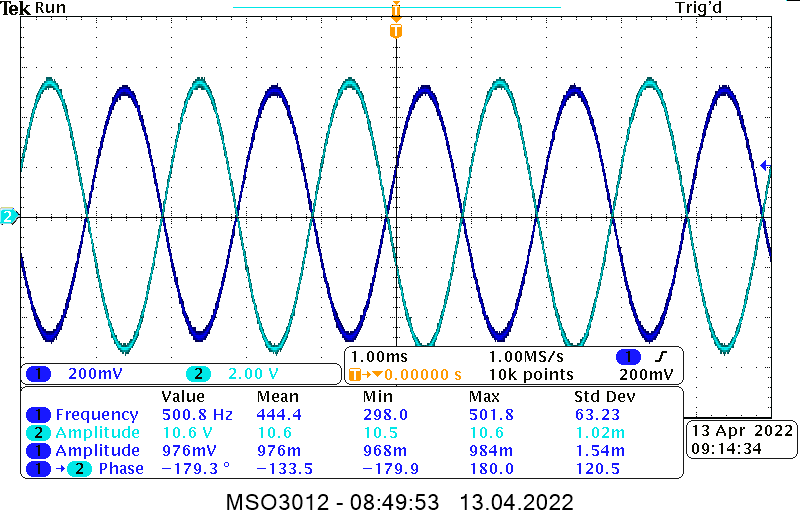
\includegraphics[width=\textwidth]{img/osciloscope/charakterystyka/1_500_cropped.png}
                \caption*{500Hz}
            \end{subfigure}
            \begin{subfigure}[h]{0.4\textwidth}
                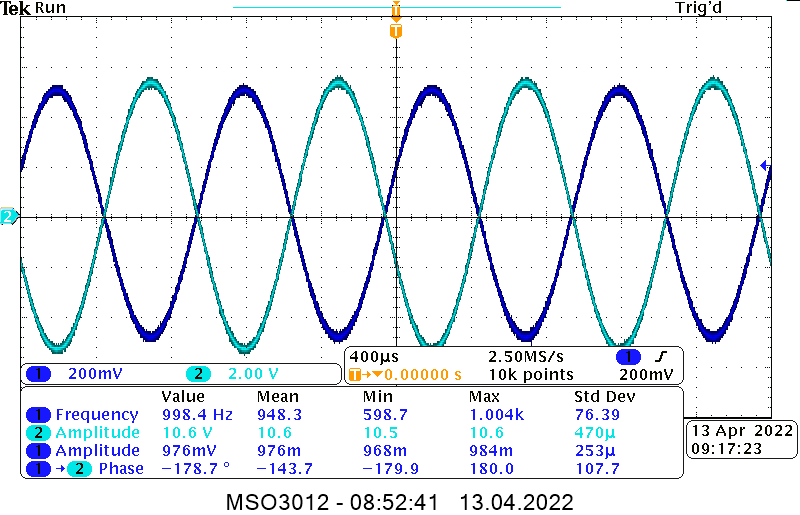
\includegraphics[width=\textwidth]{img/osciloscope/charakterystyka/1_1khz_cropped.png}
                \caption*{1kHz}
            \end{subfigure}
        \end{figure}
        
        \begin{figure}[H]
            \centering    
            \begin{subfigure}[h]{0.4\textwidth}
                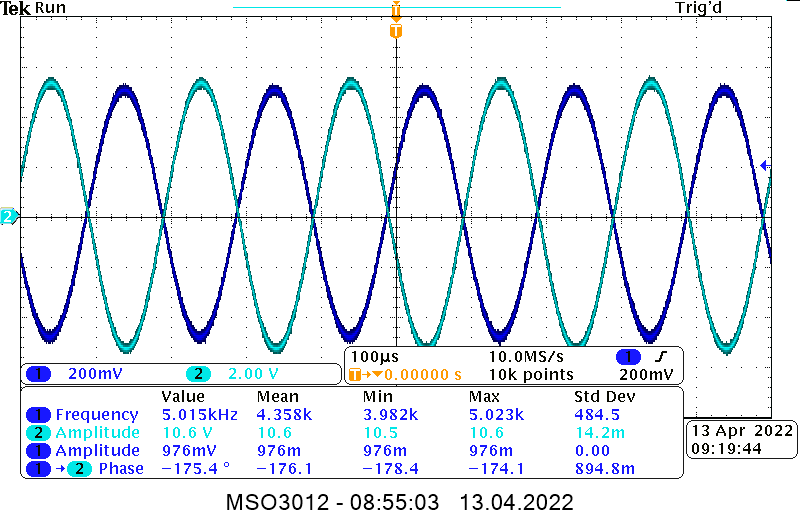
\includegraphics[width=\textwidth]{img/osciloscope/charakterystyka/1_5khz_cropped.png}
                \caption*{5kHz}
            \end{subfigure}
            \begin{subfigure}[h]{0.4\textwidth}
                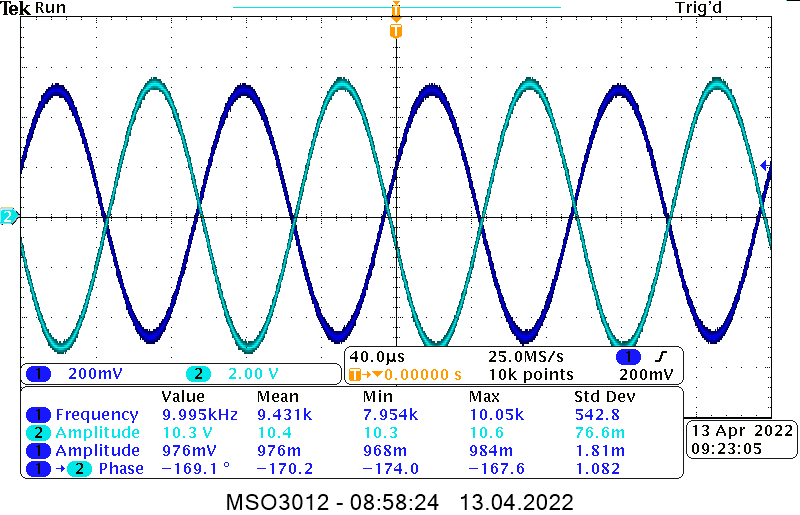
\includegraphics[width=\textwidth]{img/osciloscope/charakterystyka/1_10khz_cropped.png}
                \caption*{10kHz}
            \end{subfigure}
        \end{figure}
        
        \begin{figure}[H]
            \centering
            \begin{subfigure}[h]{0.4\textwidth}
                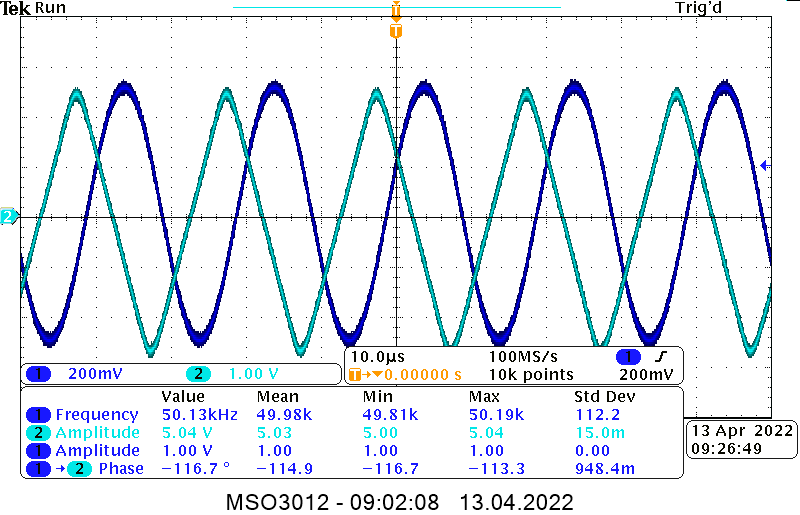
\includegraphics[width=\textwidth]{img/osciloscope/charakterystyka/1_50khz_cropped.png}
                \caption*{50kHz}
            \end{subfigure}
            \begin{subfigure}[h]{0.4\textwidth}
                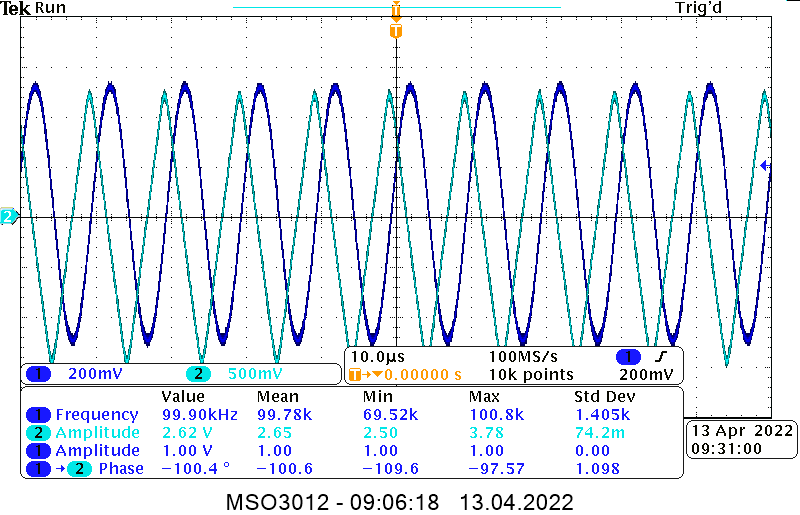
\includegraphics[width=\textwidth]{img/osciloscope/charakterystyka/1_100khz_cropped.png}
                \caption*{100kHz}
            \end{subfigure}
        \end{figure}
        
        \begin{figure}[H]
            \centering
            \begin{subfigure}[h]{0.4\textwidth}
                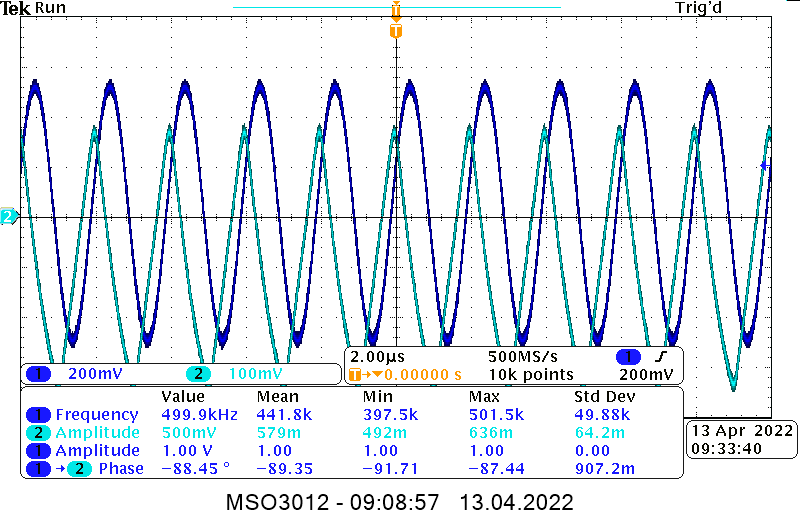
\includegraphics[width=\textwidth]{img/osciloscope/charakterystyka/1_500khz_cropped.png}
                \caption*{500kHz}
            \end{subfigure}
            \begin{subfigure}[h]{0.4\textwidth}
                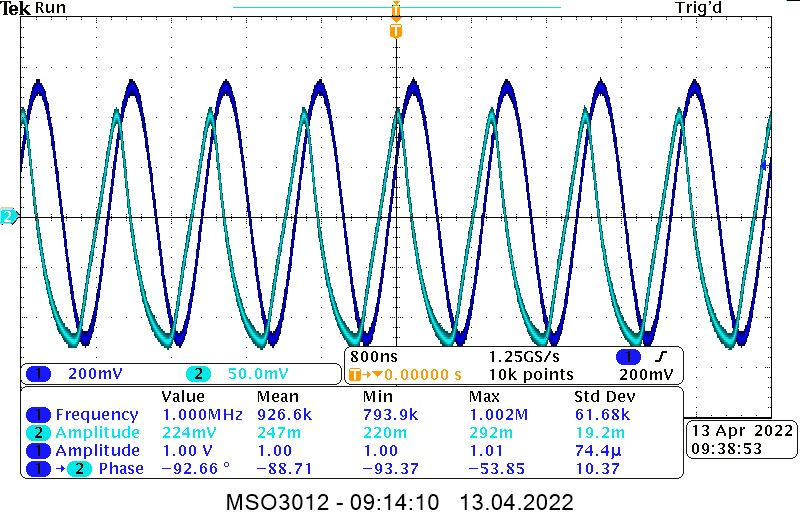
\includegraphics[width=\textwidth]{img/osciloscope/charakterystyka/1_1mhz_cropped.png}
                \caption*{1Mhz}
            \end{subfigure}
        \end{figure}
        }
    \pagebreak
    
    \item Charakterystyka amplitudowa (eksperymentalna oraz teoretyczna)
    \begin{figure}[H]
        \centering
        \begin{subfigure}[h]{0.45\textwidth}
            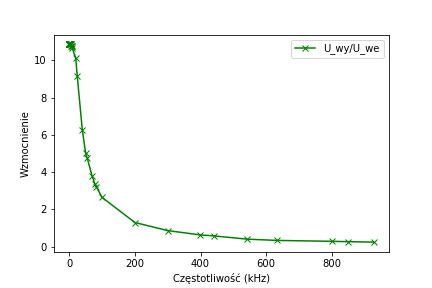
\includegraphics[width=\textwidth]{img/osciloscope/charakterystyka/uwy-we.png}
            \caption*{eksperymentalna}
        \end{subfigure}
        \begin{subfigure}[h]{0.45\textwidth}
            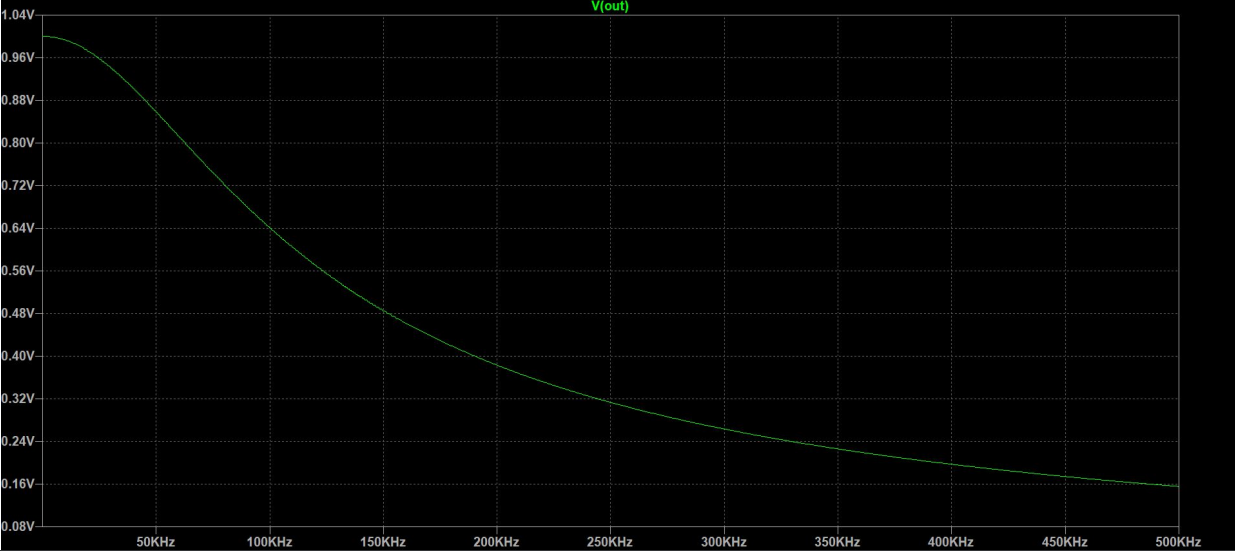
\includegraphics[width=\textwidth]{img/theoretical/charakterystyka_amplitudowa_wzmacniacz.png}
            \caption*{teoretyczna}
        \end{subfigure}
    \end{figure}
    
    \item Charakterystyka fazowa (eksperymentalna oraz teoretyczna)
        \begin{figure}[H]
        \centering
        \begin{subfigure}[h]{0.45\textwidth}
            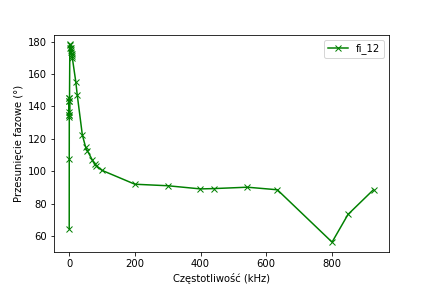
\includegraphics[width=\textwidth]{img/osciloscope/charakterystyka/fazowa.png}
            \caption*{eksperymentalna}
        \end{subfigure}
        \begin{subfigure}[h]{0.45\textwidth}
            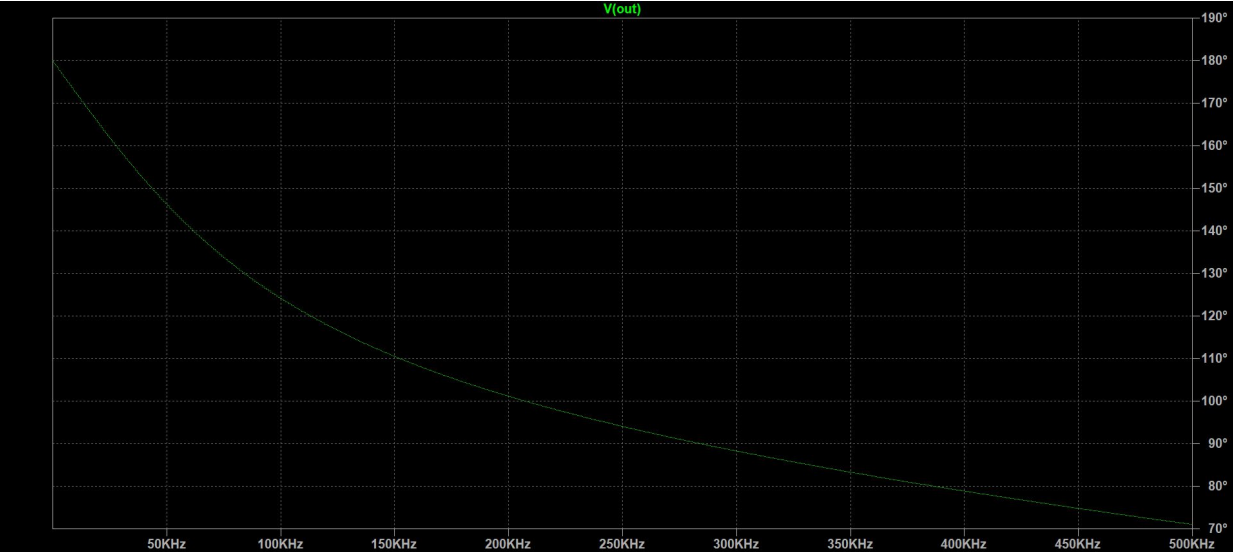
\includegraphics[width=\textwidth]{img/theoretical/charakterystyka_fazowa_wzmacniacz.png}
            \caption*{teoretyczna}
        \end{subfigure}
    \end{figure}
    \item Obie charakterystyki zgadzają się z przewidywaniami teoretycznymi, lecz widać na nich pewne odchylenia spowodowane niedokładnością pomiaru, która spowodowana może być złą kalibracją sprzętu, bądź za krótkim okresem kalibracji pomiędzy poszczególnymi pomiarami.
    \item Charakterystyka amplitudowa nie przyjmuje zamierzonego kształtu przez to, że pasmo częstotliwości jest większe.
\end{itemize}